\subsection{Algoritmos de ordenamiento}
\label{subsec:ordenamiento}

\begin{figure}[htbp]
    \centering
    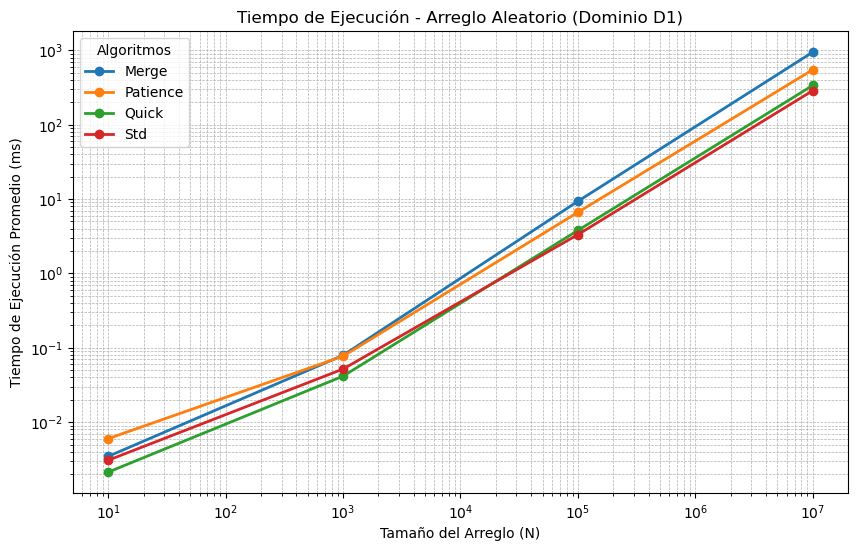
\includegraphics[width=0.48\textwidth]{../code/sorting/data/plots/tiempo_aleatorio_D1.png}
    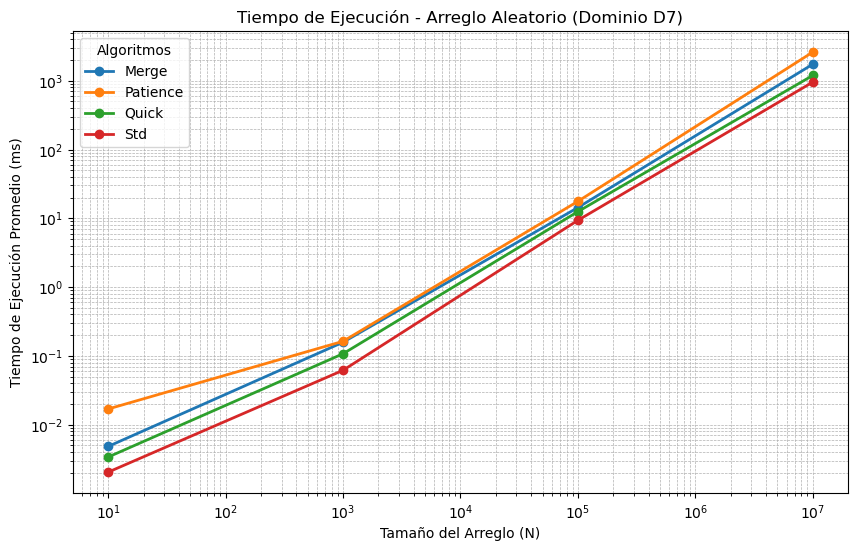
\includegraphics[width=0.48\textwidth]{../code/sorting/data/plots/tiempo_aleatorio_D7.png}
    \caption{Tiempo de ejecución para arreglos de disposición aleatoria, en el dominio $D_{1}$ (alta repetición, izquierda) y $D_{7}$ (rango amplio, derecha). Ambos ejes en escala logarítmica.}
    \label{fig:sorting_aleatorio}
\end{figure}

Los tiempos completos se encuentran en la Tabla \ref{tab:sorting_tiempo} y el consumo de memoria en la Tabla \ref{tab:sorting_memoria}. Sobre entradas aleatorias (Figura \ref{fig:sorting_aleatorio}) las cuatro curvas son aproximadamente rectas y paralelas en escala logarítmica, lo que confirma el crecimiento log-lineal común a los cuatro algoritmos; las diferencias observadas son, por tanto, diferencias de constante y no de orden de crecimiento.

\begin{itemize}
    \item \textbf{\texttt{std::sort}} obtuvo el menor tiempo en 21 de las 24 configuraciones. Las tres excepciones corresponden a QuickSort en el dominio $D_{1}$ para $N = 10^{1}$ y $N = 10^{3}$, tamaños en los que los tiempos son del orden de $10^{-2}$ ms y quedan por debajo del umbral en que la medición es distinguible del ruido. Su ventaja proviene de operar sobre memoria contigua sin estructuras auxiliares y de conmutar internamente entre \textsc{quicksort}, \textsc{heapsort} e inserción según la profundidad de recursión \cite{cppref_sort}.

    \item \textbf{QuickSort} exhibió el comportamiento teóricamente esperado sólo tras corregir el esquema de partición. La implementación inicial, que seguía el esquema de Lomuto de la referencia consultada, provocó un desbordamiento de pila (\emph{segmentation fault}) en el dominio $D_{1}$ con $N = 10^{7}$: con únicamente diez valores distintos entre diez millones de elementos, ese esquema deja todos los elementos iguales al pivote en una misma partición, la recursión degenera a profundidad $\mathcal{O}(N)$ y el costo a $\mathcal{O}(N^{2})$. Al sustituirlo por el esquema de Hoare, los índices se cruzan cerca del centro del subarreglo cuando los valores son idénticos, lo que restablece particiones balanceadas. El resultado es directamente observable: en $D_{1}$ con $N = 10^{7}$ QuickSort tarda 337{,}6 ms, es decir, 3{,}5 veces menos que en $D_{7}$ con el mismo tamaño (1\,194{,}0 ms), donde el mayor número de valores distintos impide ese balance perfecto.

    \item \textbf{MergeSort} fue el algoritmo menos sensible a la disposición inicial. Para $N = 10^{7}$ y dominio $D_{7}$, la razón entre su peor y su mejor tiempo según la disposición es de 2{,}8, frente a 4{,}7 en QuickSort, 6{,}5 en \texttt{std::sort} y 51{,}6 en PatienceSort; su consumo de memoria, además, se mantiene entre 98{,}8 y 98{,}9 MB en las seis configuraciones de ese tamaño. Ambos hechos se siguen de que su número de comparaciones y de copias depende sólo de $N$ y no del contenido de la entrada. El precio es un desplazamiento uniforme respecto de \texttt{std::sort}: unos 19 MB adicionales de memoria (98{,}8 MB frente a 79{,}7 MB) por los vectores auxiliares que asigna en cada fusión.

    \item \textbf{PatienceSort} fue el algoritmo con mayor dispersión, y su comportamiento se discute por separado a continuación.
\end{itemize}

\subsubsection*{Sensibilidad de PatienceSort a la disposición inicial}

\begin{figure}[htbp]
    \centering
    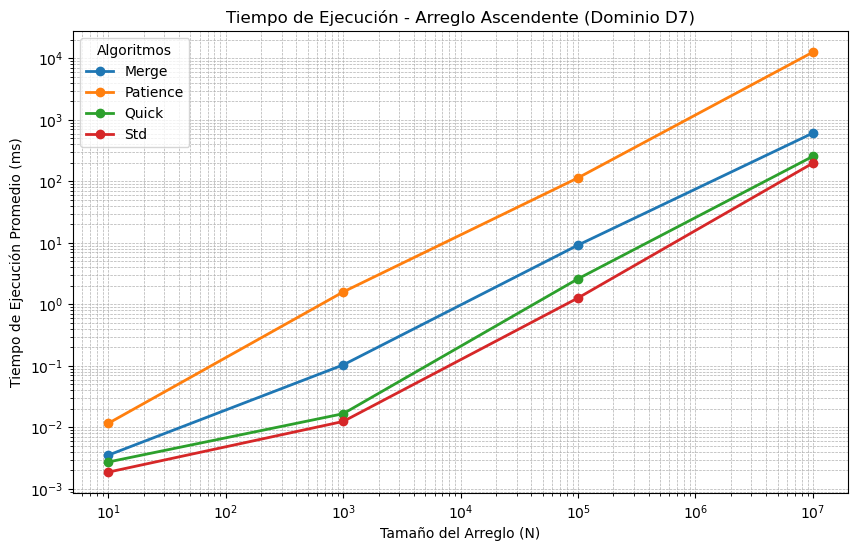
\includegraphics[width=0.48\textwidth]{../code/sorting/data/plots/tiempo_ascendente_D7.png}
    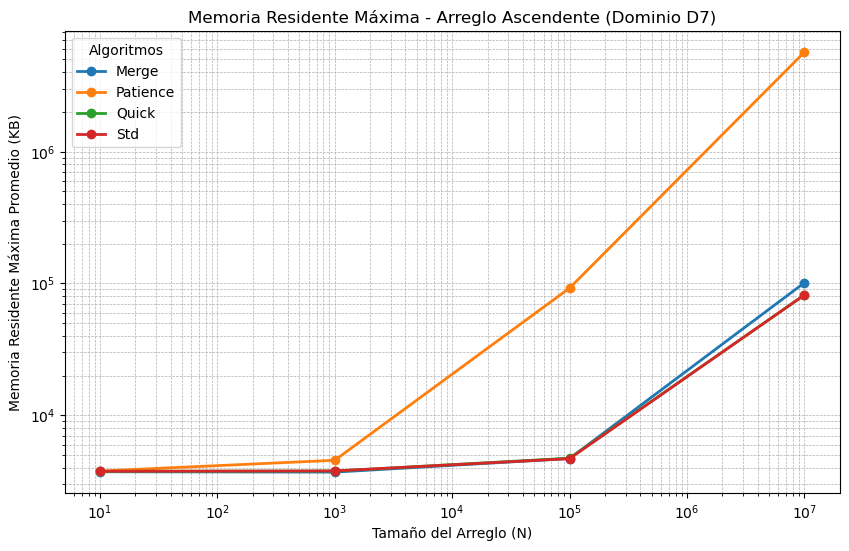
\includegraphics[width=0.48\textwidth]{../code/sorting/data/plots/memoria_ascendente_D7.png}
    \caption{Entrada ascendente en el dominio $D_{7}$: tiempo de ejecución (izquierda) y memoria residente máxima (derecha). PatienceSort se separa de los demás algoritmos en ambos ejes.}
    \label{fig:patience_ascendente}
\end{figure}

El resultado más marcado del experimento no es una diferencia de constante, sino un cambio de orden de crecimiento en el consumo de memoria. Para $N = 10^{7}$ en el dominio $D_{7}$, PatienceSort requiere 12\,629{,}7 ms y 5\,545{,}4 MB sobre una entrada ascendente, frente a 244{,}6 ms y 119{,}5 MB sobre una entrada descendente: una diferencia de 51 veces en tiempo y de 46 veces en memoria para un mismo tamaño y un mismo dominio.

La causa está en el invariante del algoritmo. Cada elemento se coloca sobre la primera pila cuyo tope sea mayor o igual a él, y crea una pila nueva si no existe tal pila. Sobre una entrada estrictamente creciente, cada elemento es mayor que todos los topes y genera una pila nueva, de modo que el número de pilas llega a igualar la cantidad de valores distintos de la entrada; sobre una entrada decreciente, todo elemento es menor o igual al tope de la primera pila y el algoritmo termina con una sola pila. El número de pilas es, en consecuencia, el largo de la subsecuencia decreciente mínima en que se descompone la entrada, y es este valor, no $N$, el que determina el costo real: la memoria auxiliar es $\Theta(\text{pilas})$ y la fusión final mantiene una cola de prioridad de ese mismo tamaño. El recuento sobre las entradas medidas lo confirma: el arreglo ascendente de $D_{7}$ contiene 6{,}32 millones de valores distintos y genera otras tantas pilas, lo que a razón de unos 900 bytes por pila --- una \texttt{std::stack} sobre \texttt{std::deque} reserva un bloque completo aunque almacene un solo entero --- da cuenta de los 5{,}5 GB observados.

El dominio confirma la explicación. Bajo $D_{1}$, donde sólo existen diez valores distintos, una entrada ascendente produce a lo sumo diez pilas, y el tiempo cae de 12\,629{,}7 ms a 328{,}4 ms y la memoria de 5\,545{,}4 MB a 144{,}1 MB. Es decir, PatienceSort no es intrínsecamente el algoritmo más lento del conjunto —en $D_{1}$ con $N = 10^{7}$ supera a MergeSort en las tres disposiciones—, sino el único cuyo costo depende de una propiedad estructural de la entrada distinta de su tamaño.

\subsection{Multiplicación de matrices}
\label{subsec:matrices}

\begin{figure}[htbp]
    \centering
    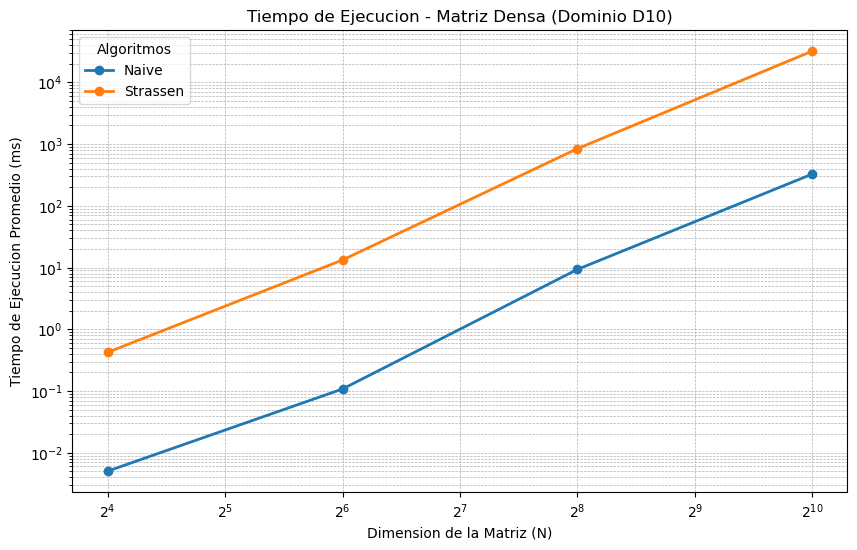
\includegraphics[width=0.48\textwidth]{../code/matrix_multiplication/data/plots/tiempo_densa_D10.png}
    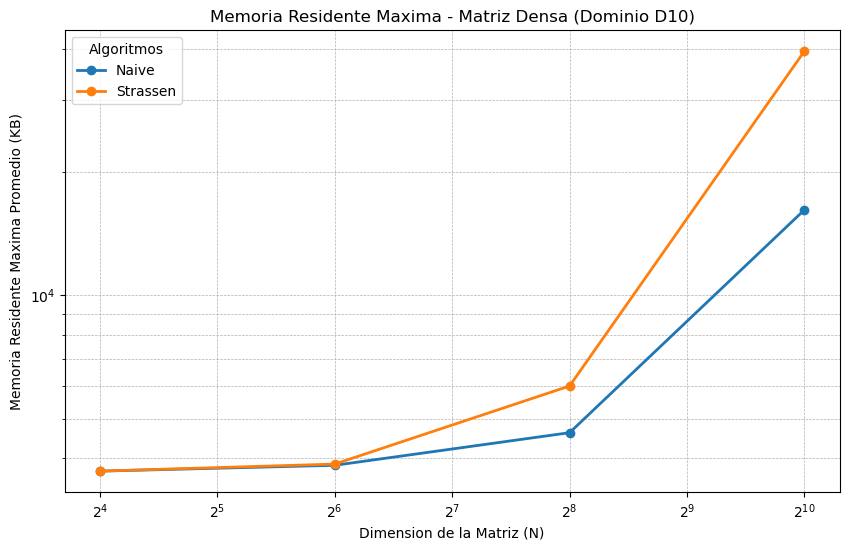
\includegraphics[width=0.48\textwidth]{../code/matrix_multiplication/data/plots/memoria_densa_D10.png}
    \caption{Matrices densas en el dominio $D_{10}$: tiempo de ejecución (izquierda) y memoria residente máxima (derecha) para los algoritmos Naive y Strassen.}
    \label{fig:matrix}
\end{figure}

Las mediciones completas se presentan en la Tabla \ref{tab:matrix_mediciones}. Antes de interpretarlas es necesario acotar la precisión del experimento: para $N = 1024$, las 18 ejecuciones individuales del algoritmo Naive, que realizan exactamente el mismo número de operaciones aritméticas, arrojan tiempos entre 242{,}8 y 749{,}0 ms. Cualquier diferencia inferior a un factor de tres en esta escala es, por tanto, atribuible a la variabilidad del entorno y no al algoritmo.

\begin{itemize}
    \item \textbf{Sobrecarga de la recursión pura:} Como ahora forzamos a Strassen a dividirse hasta el final (matrices de $1 \times 1$) sin usar el método tradicional como caso base, el rendimiento se desploma. Aunque en teoría Strassen hace menos multiplicaciones, el tener que crear y destruir tantos vectores dinámicos en cada nivel de la recursión genera un cuello de botella enorme, haciéndolo muchísimo más lento que el método tradicional para matrices chicas ($N \le 64$).

    \item \textbf{El cruce asintótico que no ocurrió:} Esperábamos que en la dimensión mayor ($N = 1024$) Strassen fuera más rápido por su menor complejidad teórica ($\mathcal{O}(N^{2,81})$ vs $\mathcal{O}(N^3)$). Sin embargo, pasó todo lo contrario: la sobrecarga de pedir y liberar memoria ahogó al procesador. Strassen terminó siendo unas 118 veces más lento que Naive (tardó casi 31 segundos frente a los 0,26 segundos del método tradicional). En la práctica, hacer recursión pura hasta el fondo mata cualquier ventaja matemática a esta escala.

    \item \textbf{Costo en memoria de la recursión.} La ventaja en tiempo se paga en espacio. Para $N = 1024$, Strassen ocupa 38{,}6 MB frente a los 15{,}8 MB del algoritmo iterativo, un factor de 2{,}4, producto de las submatrices y resultados intermedios que cada uno de los cuatro niveles de recursión mantiene vivos simultáneamente. Esta diferencia, a diferencia de las de tiempo, es reproducible entre ejecuciones y crece con $N$.

    \item \textbf{Ausencia de efecto de la dispersión.} Ambas implementaciones almacenan las matrices como arreglos densos y ejecutan la misma aritmética sobre los coeficientes nulos, por lo que no cabe esperar ganancia alguna en las matrices dispersas o diagonales. Las mediciones son consistentes con esta predicción: las diferencias observadas entre tipos de matriz para un mismo algoritmo y tamaño caen dentro del margen de ruido establecido más arriba. Aprovechar la dispersión exigiría una representación comprimida, como el formato CSR, lo que constituye un cambio de estructura de datos y no de algoritmo.
\end{itemize}
